\chapter{Implementazione del ChatBot}
\label{chatbot}

Per apprendere il funzionamento dei token \emph{JWT} e dei vari metodi di autenticazione, è stato richiesto di implementare un \emph{ChatBot} per la piattaforma \emph{Microsoft Teams} che si interfacciasse con i servizi \emph{API} dell'azienda.
L'intero codice è stato scritto in \emph{C\#} e utilizzando il framework \emph{.NET Core 8.0}.

\begin{figure}[!ht]
    \centering
    \begin{minipage}[t]{0.5\textwidth}
        \centering
        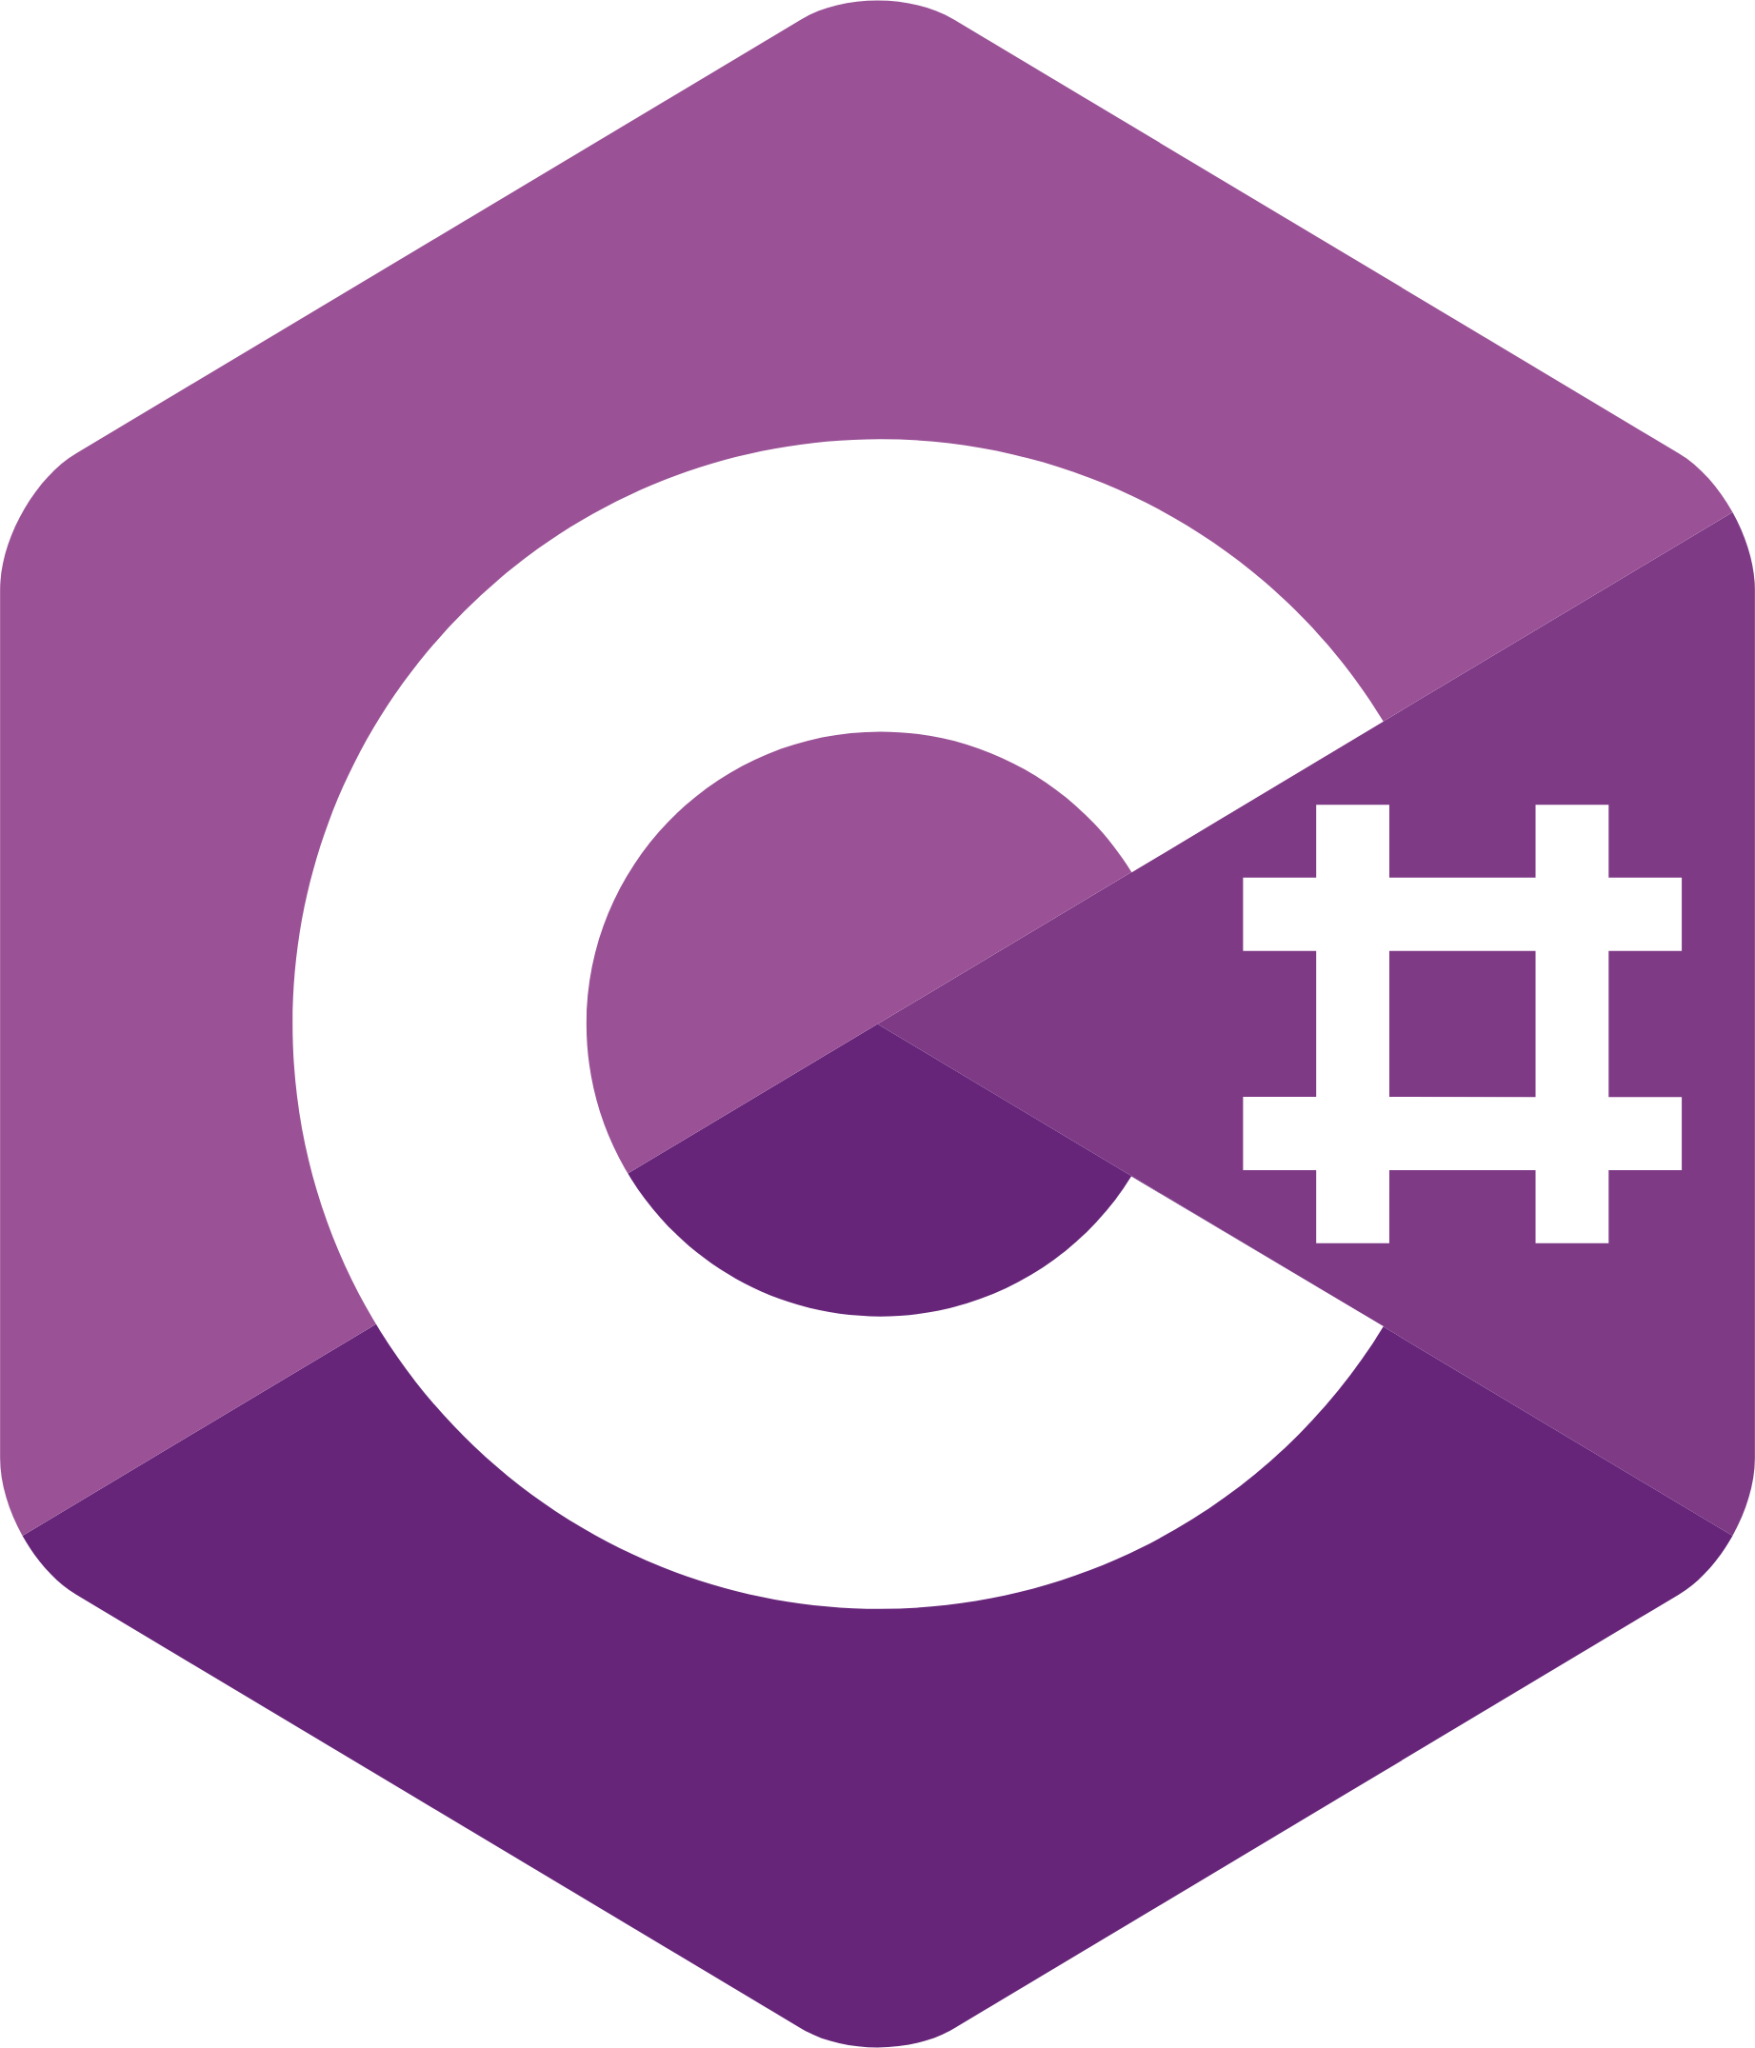
\includegraphics[width=0.25\textwidth]{chatbot/csharp-icon}
        \caption{Logo di C\#}
    \end{minipage}\hfill
    \begin{minipage}[t]{0.5\textwidth}
        \centering
        
\includegraphics[width=0.25\textwidth]{chatbot/dotnet-icon}
        \caption{Logo di .NET Core}
    \end{minipage}
\end{figure}

